% =====================================================================
% datos_reales.tex
% Responsabilidad única: contar qué encontramos al pasar a la exportación
% real del laboratorio (solo fechas de desarrollo): lotes de Poisson,
% muestras como Poisson compuesta, tamaño de lote por tipo, segmentos,
% riesgo al ingreso y distancia con la simulación.
% Cifras: macros Real*; tablas tabla_real_*; figuras 08_*.
% Si la exportación no estaba al construir, las macros Real* no existen y
% la sección se reduce a una nota.
% =====================================================================
\section{Datos reales: Lotes de Poisson}
\label{sec:datos-reales}

\ifdefined\RealMuestras
Al final del semestre Daniel Arias Mutis, que trabaja en el laboratorio,
consiguió la exportación real con los clientes anonimizados. Nos propuso
clasificar a los clientes por su volumen y a los lotes por su tamaño y nos
dijo que las llegadas le sonaban a un proceso de Poisson. Solo usamos las
fechas de desarrollo (del \RealDesde{} al \RealHasta{}) y dejamos por fuera
todo lo de 2026, que además es donde la base empieza a cambiar. Las
\RealFilas{} filas de la exportación (una por muestra, especificación y
lectura) se vuelven \RealMuestras{} muestras de \RealClientes{} clientes y
\RealLotes{} lotes, donde un lote son las muestras que un cliente ingresa el
mismo día y del mismo tipo (producto o muestreo en planta). El
\RealPlantaPct{}\,\% de las muestras viene de planta y la no conformidad es
de \RealNoConformePct{}\,\%.

\paragraph{Muestras y lotes.} En una Poisson la varianza es igual a la media
así que medimos el índice de dispersión $I = s^2/\bar x$ de los conteos
semanales de cada cliente. Esperábamos que las muestras por semana dieran
cerca de 1 y no fue así: Con los \RealClientesDispersion{} clientes que
tienen al menos \RealMinimoLotes{} lotes la mediana del índice es de
\RealDispMuestrasTodos{} y llega hasta \RealDispMuestrasMax{}. Al contar
lotes en vez de muestras la mediana baja a \RealDispLotesTodos{}
(Figura~\ref{fig:real-dispersion}). Por tipo el índice de los lotes es de
\RealDispLotesProducto{} en producto y \RealDispLotesPlanta{} en planta,
frente a \RealDispMuestrasProducto{} y \RealDispMuestrasPlanta{} en las
muestras (Tabla~\ref{tab:real-dispersion}).

\begin{figure}[!htbp]
\centering
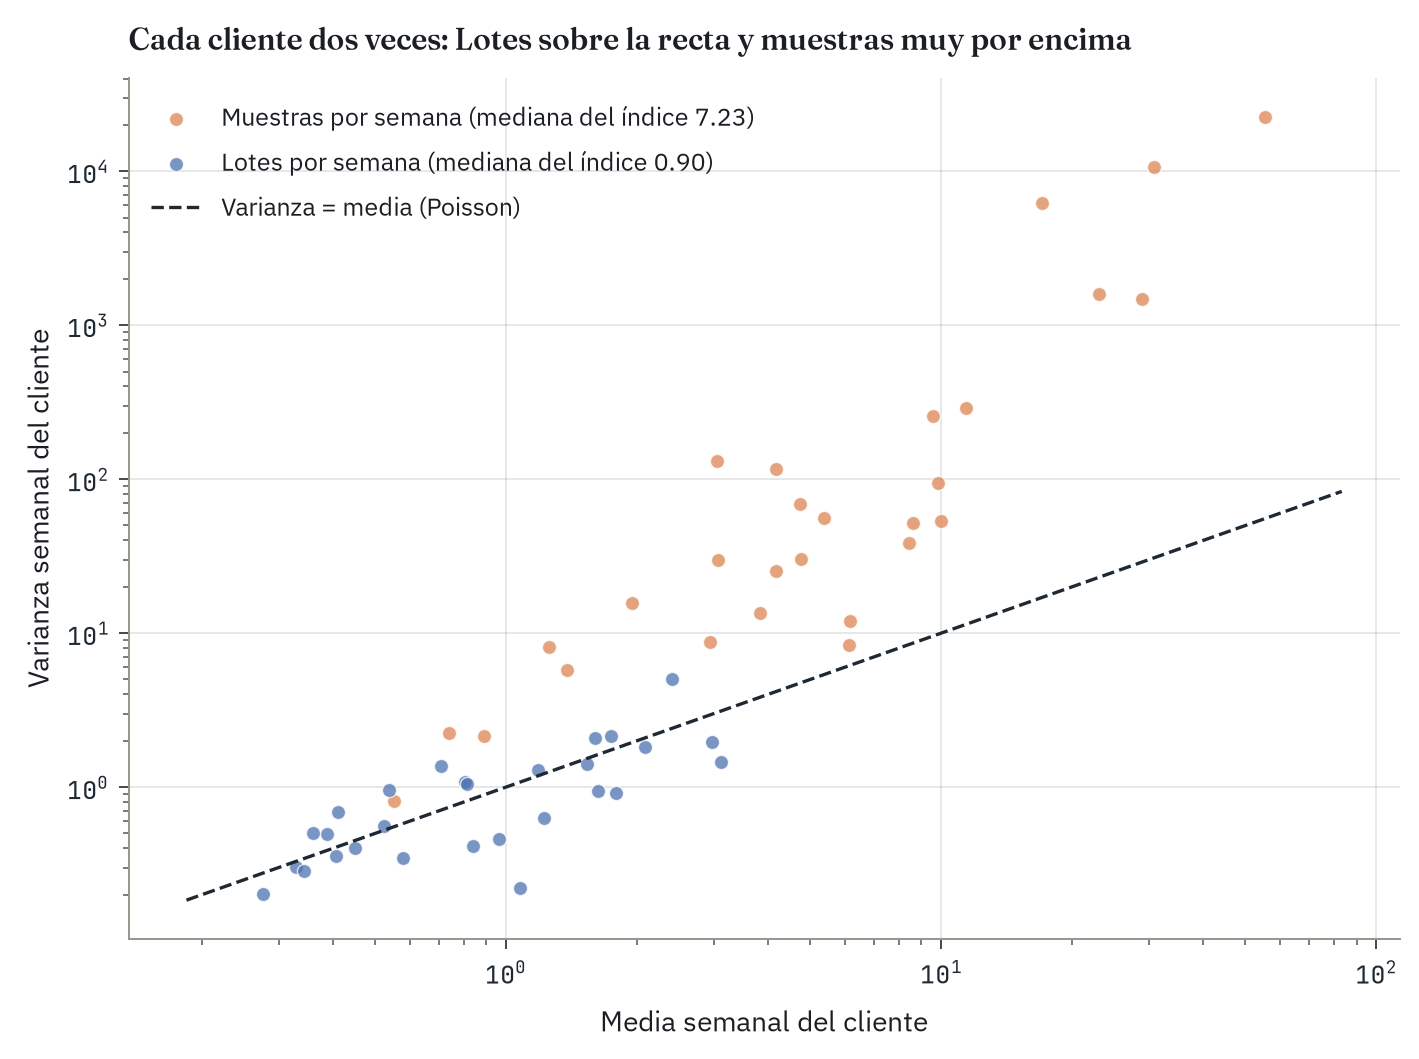
\includegraphics[width=0.7\textwidth]{08_dispersion_clientes.png}
\caption{Media frente a varianza semanal de cada cliente, una vez con sus
muestras y otra con sus lotes, en ejes logarítmicos: Los lotes caen sobre la
recta de Poisson y las muestras quedan muy por encima.}
\label{fig:real-dispersion}
\end{figure}

\begin{table}[!htbp]
\centering
\tablaancha{real_dispersion}
\caption{Índice de dispersión semanal por cliente y tipo de lote, con la
proporción de clientes en que la prueba de dispersión da un valor p menor
que \RealNivel{}: La sobredispersión está en las muestras y no en los lotes.}
\label{tab:real-dispersion}
\end{table}

La explicación es que las muestras son una Poisson compuesta: Si llegan
$N \sim \mathrm{Poisson}(\lambda)$ lotes y el lote $i$ trae $X_i$ muestras,
el total $S = \sum_{i=1}^{N} X_i$ tiene $E[S] = \lambda E[X]$ y
$\mathrm{Var}[S] = \lambda E[X^2]$, de modo que su índice es
$E[X^2]/E[X]$ y crece con la variación del tamaño de lote. Con los lotes de
cada cliente esa cuenta da medianas de \RealCompuestoProducto{} en producto y
\RealCompuestoPlanta{} en planta, del mismo orden que lo observado.

\paragraph{Tamaño de lote.} Modelamos el tamaño como uno más un conteo y
comparamos con el AIC tres opciones (Tabla~\ref{tab:real-tamano} y
Figura~\ref{fig:real-tamano}). En producto los lotes son pequeños (media
\RealLoteMediaProducto{}, mediana \RealLoteMedianaProducto{}) y gana la
\RealLoteMejorProducto{} con $r = \RealLoteRProducto$, aunque la geométrica
queda a solo \RealLoteDeltaGeoProducto{} de AIC. En planta la media es
\RealLoteMediaPlanta{}, la mediana \RealLoteMedianaPlanta{} y el máximo
\RealLoteMaxPlanta{} muestras en un día así que la cola larga de la
\RealLoteMejorPlanta{} ($r = \RealLoteRPlanta$) le saca
\RealLoteDeltaGeoPlanta{} de AIC a la geométrica. Las \RealCampanas{}
campañas de muestreo en planta duran casi siempre un solo día
(\RealCampanaUnDiaPct{}\,\%).

\begin{figure}[!htbp]
\centering
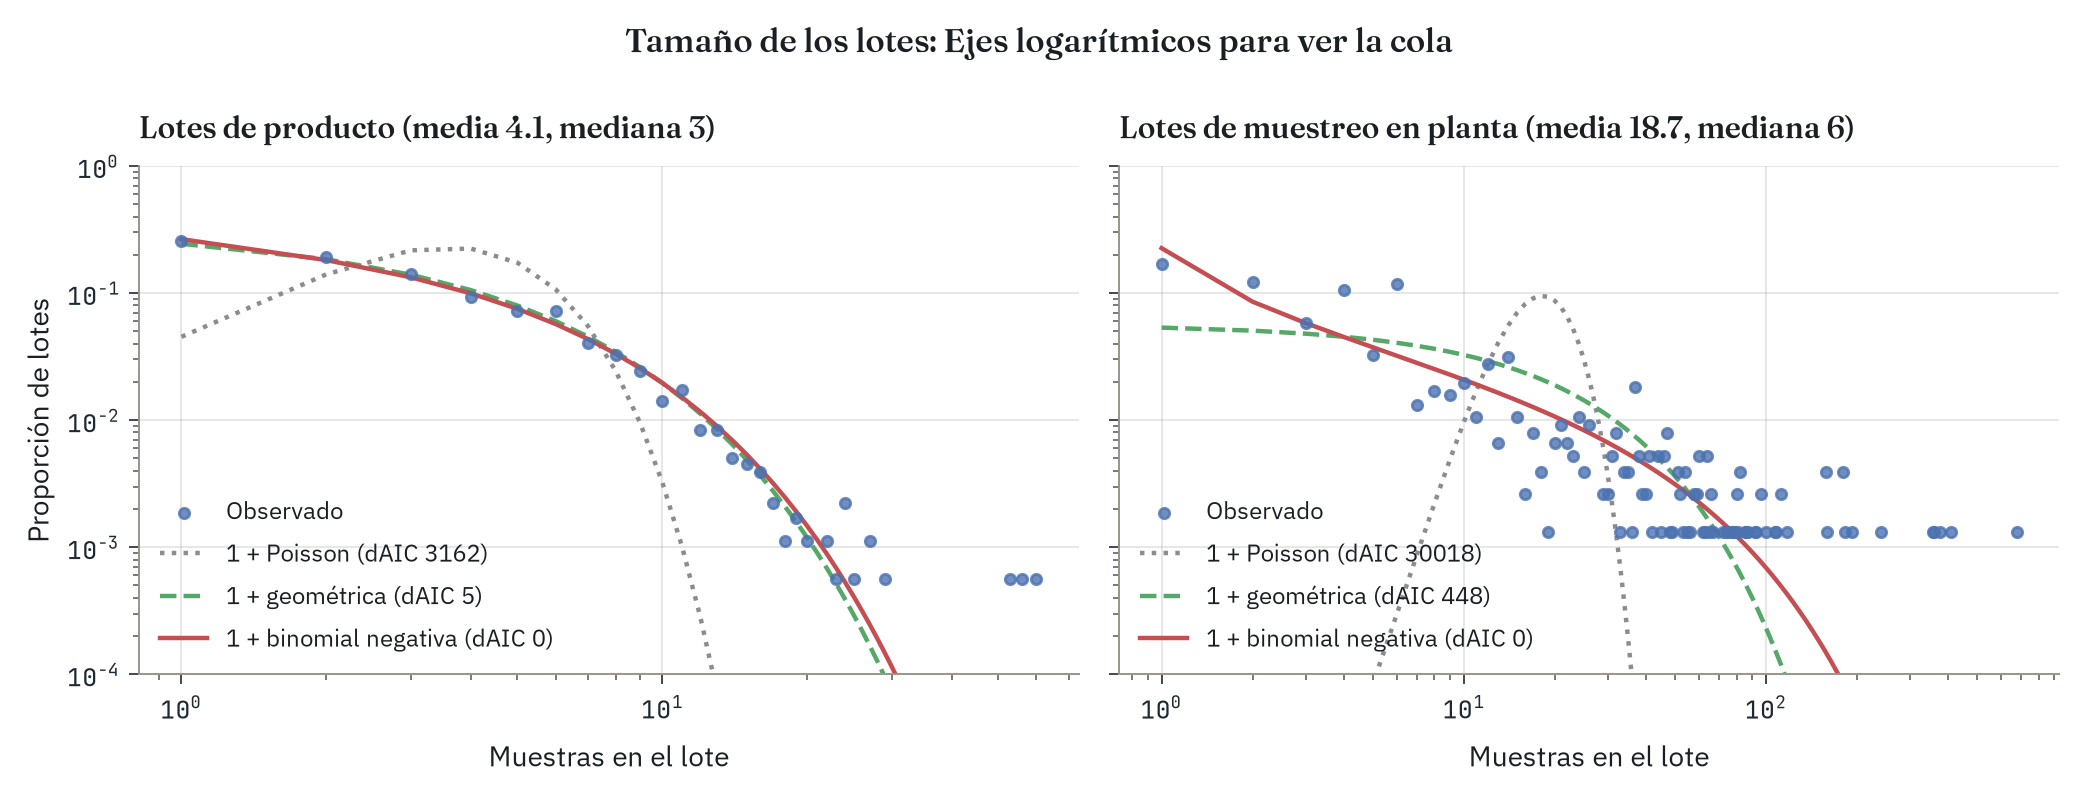
\includegraphics[width=\textwidth]{08_tamano_lote.png}
\caption{Proporción de lotes de cada tamaño con los tres modelos ajustados,
en ejes logarítmicos: Uno más una Poisson no alcanza la cola en ningún tipo y
la binomial negativa sigue los datos.}
\label{fig:real-tamano}
\end{figure}

\begin{table}[!htbp]
\centering
\tablaancha{real_tamano_lote}
\caption{Modelos del tamaño de lote por tipo: La binomial negativa tiene el
menor AIC en los dos.}
\label{tab:real-tamano}
\end{table}

\paragraph{Segmentos y riesgo.} Con el procedimiento de la
Sección~\ref{sec:agrupamiento} sobre \RealSegClientes{} clientes (al menos
\RealSegMinimoMuestras{} muestras) la silueta eligió \RealSegK{} segmentos
(silueta \RealSegSilueta{}). El que más pesa es ``\RealSegMayor'', que trae
el \RealSegMayorMuestrasPct{}\,\% de las muestras. Para el riesgo de no
conformidad al ingreso ajustamos en entrenamiento y medimos en validación
(prevalencia de \RealRiesgoPrevalenciaPct{}\,\%): La regresión logística da
un ROC-AUC de \RealRiesgoAUCLogistica{} (precisión media
\RealRiesgoAPLogistica{}) y el árbol \RealRiesgoAUCArbol{}
(\RealRiesgoAPArbol{}), frente a \RealRiesgoAPBase{} de precisión media de la
línea base. La tasa histórica del cliente sola ya logra
\RealRiesgoAUCHistoria{} así que la señal es real pero modesta.

\paragraph{La simulación.} Nuestra simulación ya generaba lotes de Poisson
con varias muestras cada uno así que la estructura era la correcta. Lo que no
reproduce es el tamaño: Con uno más una Poisson el índice de las muestras
queda entre \RealSimIndiceBajo{} y \RealSimIndiceAlto{}, lejos de la cola de
planta. Separar producto y planta y sacar el tamaño de una binomial negativa
la acercaría. Lo dejamos propuesto porque las secciones anteriores están
cerradas sobre la simulación actual.
\else
Esta versión del informe se construyó sin la exportación real del
laboratorio (el archivo es confidencial y no viaja con el proyecto) así que
la sección no tiene cifras.
\fi
